\chapter{Botnets}
As Botnets são redes formadas por máquinas infectadas com malware, permitindo que o botmaster (o atacante) realize diversas atividades criminais remotamente, como roubo de informações, ataques de negação de serviço, envio de SPAM, etc.\cite{silva2013botnets}

Com o crescimento e diversificação do uso da Internet, o meio cibernético se tornou mais relevante e mais atraente para a realização de ataques maliciosos. Isso motivou o crescimento do número de botnets existentes e aumentou o potencial de contaminação das mesmas, além disso, para evitar os mecanismos de detecção existentes, elas se tornaram cada vez mais sofisticadas.

Para que o detector se torne mais robusto, e leve em conta as configurações existentes e até detecte possíveis novas configurações das botnets, é preciso compreender o funcionamento das botnets e seus objetivos, para que possamos identificar características constantes na botnet, mesmo quando o botmaster está tentando evitar os mecanismos de detecção.

\section{Elementos das Botnets}
Estruturalmente, as botnets são formadas pelos bots, que são malwares instalados nos computadores das vítimas que podem realizar as ações maliciosas que o botmaster envia através do canal de comando e controle (C\&C). Geralmente, o malware é inicializado quando o hospedeiro inicializa a máquina, porém isso pode ser configurado pelo botmaster para dificultar a detecção da atividade maliciosa.

O canal de C\&C é o meio que o botmaster tem para se comunicar com a sua botnet, e é a parte chave do funcionamento, pois é necessário para o envio dos comandos necessários para a atividade maliciosa aos hospedeiros. Dessa forma, grande parte das características da botnet, como robustez, facilidade de detecção/desativação, estabilidade, etc., são definidas pela forma que a infraestrutura de C\&C está organizada.

\section{Ameaças e Formas de Defesa}
O crescimento do número de máquinas conectadas constantemente à enlaces de alta velocidade e rodando sistemas com vulnerabilidades consideráveis, criou um ambiente favorável à formação de botnets. Esse crescimento, aliado à alta efetividade e potencial de causar danos, fez com que as botnets se tornassem um dos maiores desafios de pesquisa em segurança no espaço cibernético atual. \cite{soltani2014survey}

Existem características que tornam o host mais interessantes ao botmaster como: altas taxas de transmissão, baixos níveis de segurança e monitoração, alta disponibilidade e localização distante (dificultando que as agências reguladoras detectem as atividades, já que os bots estarão espalhados por diversas nações). Esses fatores ajudam o bot a passar desapercebido e a contribuir com maior capacidade de banda ao botmaster, facilitando ataques como os de negação de serviço.

Existem duas formas para o combate das botnets: reativamente ou preventivamente. A forma reativa é a mais comum e envolve detectar a existência da botnet e reagir ao ataque tentando reduzir o tráfico malicioso para níveis aceitáveis, uma desvantagem é que o ataque já vai ter sido inicializado quando for detectado, ou seja, já vai haver causado danos antes de ser solucionado. A forma preventiva busca evitar que a botnet possa realizar alguma atividade maliciosa, porém essa atividade não é simples, já que o atacante pode aprimorar seus bots, tornando os mais sofisticados, exigindo grandes investimentos para manter os recursos de segurança atualizados.

O mecanismo que estamos desenvolvendo é da forma reativa, já que o algoritmo encontrará padrões em botnets que já estão atuando. Porém, uma característica desejável para um detector reativo é a detecção em tempo real, com o objetivo de minimizar os danos causados e o tempo de reação do botmaster. Porém, essa característica é um desafio, devido ao grande número de dados que devem ser tratados e analisados. Dessa forma, nosso objetivo neste projeto será se aproximar disso, utilizando a detecção dos dados coletados ao longo de um dia para detectar bots que atuaram nas últimas 24 horas.

\section{Ciclo de Vida das Botnets}
Na maioria dos casos, existe um ciclo com fases bem definidas de como uma botnet é criada e mantida, a Figura \ref{fig:botnets_lifecycle} mostra essas fases para cada novo hospedeiro que é contaminado. 

Na primeira fase, chamada de injeção inicial, o atacante procura vulnerabilidades na máquina do futuro hospedeiro para explorá-las e infecta-lo com o malware, tornando-se um bot em potencial, isso pode ocorrer, por exemplo, através de um download indesejado ou através de um anexo em um e-mail. Após a infecção ser bem sucedida, ocorre a injeção secundária: o host infectado, através do malware inicial instalado, busca em uma rede os reais binários do malware do bot, os quais após baixados e executados concluirão a infecção e tornam o host em um bot real.\cite{feily2009survey}.

Durante a fase de conexão, o bot estabelece conexão com o canal de C\&C, isso se repete sempre que o host é reiniciado, podendo ser considerada uma fase vulnerável já que segue um padrão. Após a efetivação da conexão, o bot se torna ativo na botnet, e passa a realizar os comandos enviados pelo botmaster através do canal de C\&C, efetivando as atividades maliciosas solicitadas. A última fase é a de manutenção e atualização, e tem por objetivo manter a botnet ativa e atualizada, já que se o botmaster deseja que os bots possam evitar novas técnicas de detecção, adicionar novas funcionalidades ou até mesmo alterar o servidor de C\&C, os binários do programa bot devem ser modificados.

\tikzstyle{block} = [rectangle, draw, text width=9em, text centered, rounded corners, minimum height=4em]
\tikzstyle{line} = [draw, -latex']

\begin{figure}
\centering
\begin{tikzpicture}[node distance = 4.5cm, auto]
    % Place nodes
    \node [block] (init) {Infecção Inicial};
    \node [block, below of=init] (second) {Injeção Secundária};
    \node [block, right of=init] (connection) {Conexão};
    \node [block, below of=connection] (malicious) {Atividades Maliciosas};
    \node [block, right of=malicious] (update) {Manutenção e Atualização};
    % Draw edges
    \path [line] (init) -- (second);
    \path [line] (second) -- (connection);
    \path [line] (connection) |- +(4,2) |- (connection.east); 
    \path [line] (connection) -- (malicious);
    \path [line] (malicious) -- (update);
    \path [line] (update) -- (connection);

\end{tikzpicture}
\caption[Ciclo de Vida das Botnets]{Ciclo de Vida das Botnets} \label{fig:botnets_lifecycle}
\end{figure}

\section{Arquitetura das Botnets}
Existem 4 tipos de arquiteturas para as botnets: centralizada, descentralizada, híbrida e aleatória. 

Na arquitetura centralizada, mostrada na figura \ref{fig:centralized_architecture} todos os bots se comunicam com um número pequeno de servidores de C\&C, embora ela ofereça vantagens ao botmaster, como baixa latência e facilidade de manutenção, ela também torna a botnet bastante vulnerável, permitindo que ela seja desligada após a identificação dos poucos pontos centrais de C\&C. Ela é muito utilizada pelo protocolo IRC (\textit{Internet Relay Chat}), porém pelo fato de tráfego desse protocolo ser incomum e raramente utilizado, ele costuma ser bloqueado, inutilizando a botnet. Por isso, o uso do protocolo HTTP (\textit{HyperText Transfer Protocol}) se popularizou já que ele é muito utilizado, disfarçando as comunicações das botnets.

Isso motivou o desenvolvimento da arquitetura descentralizada, onde uma variedade de protocolos P2P é utilizada, permitindo que mesmo que muitos bots sejam desativados a botnet possa continuar funcionando, já que não existem pontos centralizados de C\&C. A arquitetura híbrida apresenta características de ambas as arquiteturas centralizadas e descentralizadas, na qual os bots são classificados em dois grupos: clientes e servos, os servos exercem os papéis tanto de clientes quanto servidores, sendo utilizados para repassar os comandos enviados pelo botmaster. Por fim, a arquitetura aleatória é um modelo apenas teórico, no qual o bot não se comunica ativamente com o botmaster ou com outros bot, para realizar um ataque o botmaster vasculha a rede em busca de um bot para enviar o comando e realizar as atividades maliciosas.

\begin{figure}
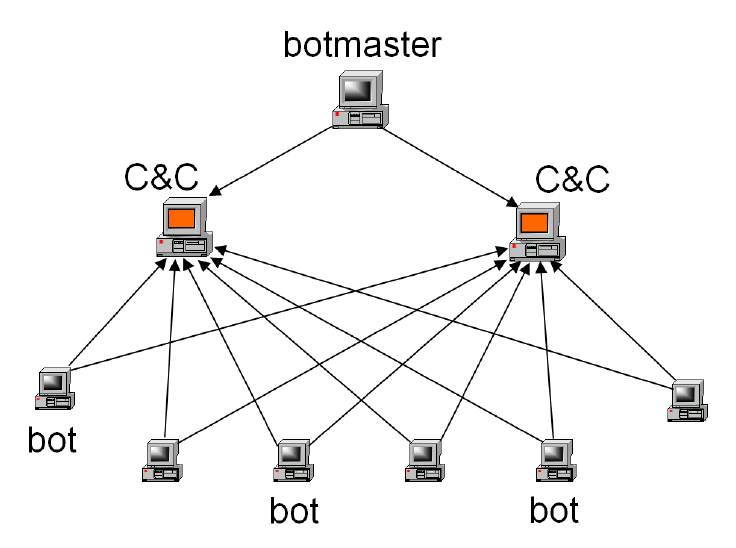
\includegraphics[width=\textwidth]{centralized}
\caption[Arquitetura Centralizada]{Arquitetura Centralizada\cite{wang2010advanced}} \label{fig:centralized_architecture}
\end{figure}

\begin{figure}
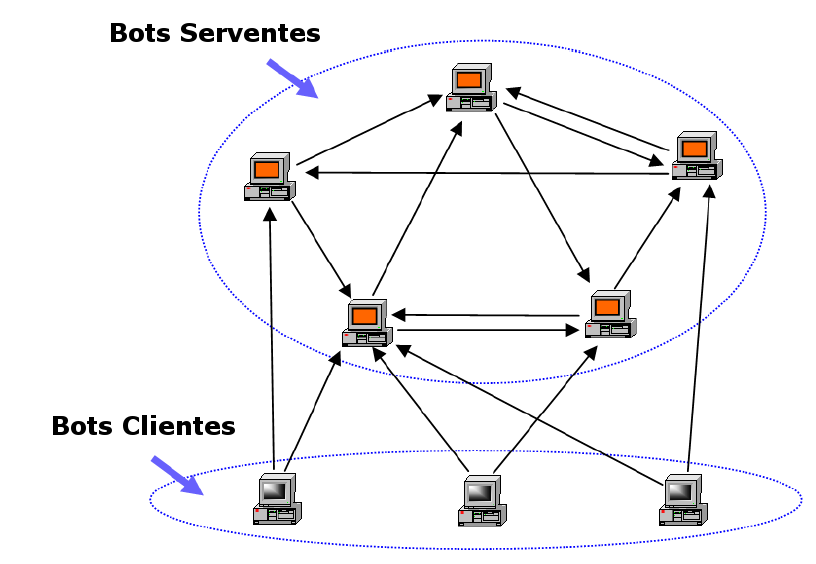
\includegraphics[width=\textwidth]{hybrid}
\caption[Arquitetura Híbrida]{Arquitetura Híbrida\cite{wang2010advanced}} \label{fig:hybrid_architecture}
\end{figure}

\section{Detecção de Botnets}

Existem duas categorias de técnicas para detecção de botnets: honeynets e sistemas de detecção de intrusos (IDS). As honeynets consistem na criação de redes com a intenção de que elas sejam comprometidas, permitindo que as informações sobre a botnet sejam captadas.

A detecção via IDS, pode ser classificada entre duas técnicas: a baseada em assinaturas e a baseada em anomalias. A técnica baseada em assinaturas, consiste em extrair padrões da rede e comparar com um banco de dados onde se encontram os padrões que já foram vistos em botnets, ou seja, ela não permite que novas botnets sejam identificadas. Dessa forma, a técnica baseada em anomalias é a principal área de pesquisa para detecção de botnets, baseando-se em anomalias na rede, como alta latência, aumento no tráfego ou uso de portas incomuns para detectar a presença de bots na rede.

As técnicas baseadas em anomalias, podem ser baseadas no host, onde cada máquina possui uma ferramenta de monitoração instalada (o que não é muito escalável), e tem seu comportamento analisado para verificar a existência de atividades suspeitas. Além disso, a análise pode ser baseada na rede, ativa (que possuem a grande desvantagem de aumentar o tráfego da rede ao injetar pacotes com a finalidade de examinar se um cliente é humano ou um bot) ou passivamente, sendo a forma de detecção mais utilizada atualmente.

A monitoração passiva de uma rede consiste em analisar o tráfego da rede buscando por comunicações suspeitas que podem ter sido enviadas pelos bots ou canais de C\&C. Essa monitoração é possível pois os bots de uma mesma botnet costumam apresentar padrões de comunicação, já que eles são pré-programados pelo mesmo botmaster para entrar contato com o servidor de C\&C.

Para que a análise do tráfego seja viabilizada, são empregadas diversas técnicas como métodos estatísticos, mineração de tráfego, teoria de grafos, clustering, modelos estocásticos, redes neurais, entre outras.

A detecção de botnets é uma tarefa bastante desafiadora porque os botmasters estão sempre aprimorando os bots, tornando os mais difíceis de serem detectados. Por exemplo, as primeiras detecções buscavam mensagens suspeitas nos conteúdos da mensagem, afim de evitar isso os botmasters passaram a utilizar criptografia tornando essa técnica de detecção obsoleta. Outra dificuldade para algoritmos de clustering é que podem ser evitados usando técnicas de randomização nas comunicações e atribuição de tarefas diferentes para os bots.

\section{Sistema Integrado de Defesa Cibernética para Detecção de Botnets}
Em \cite{silva2012arquitetura} foi proposta a.
